\documentclass[5]{article}
\usepackage[utf8]{inputenc}
\usepackage{hyperref} 

\usepackage[T1]{fontenc}
\usepackage[polish]{babel}

\title{Laboratorium 3}
\author{Piotr Witek}
\date{24 marca 2021}

\usepackage{natbib}
\usepackage{graphicx}
\usepackage{geometry}
\usepackage{tabularx}
\usepackage{array}
\usepackage{amsmath}

\begin{document}

\newgeometry{tmargin=2cm, bmargin=2cm, lmargin=2.5cm, rmargin=2.5cm}

\maketitle

\section{Zadania}

\subsection{Aproksymować funkcję $f(x) = 1+ x^{3}$ w przedziale [0,1] wielomianem pierwszego stopnia metodą średniokwadratową ciągłą dla w(x)=1.}


Aproksymujemy wielomianami $\phi_{n}(x)=x^{n}$, więc funkcja aproksymująca ma postać:
$$
F(x)=\sum_{i=0}^{n} c_{i} \phi_{i}(x), c_{i} \in \mathbb{R}
$$
Odległość od funkcji aproksymowanej w metryce $L_{1}^{2}([0,1])$ wynosi:
$$
\delta(f, F)=\int_{0}^{1}[F(x)-f(x)]^{2} d x=\int_{0}^{1}\left[\sum_{i=0}^{n} c_{i} \phi_{i}(x)-f(x)\right]^{2} d x
$$
Aby znaleźć minimum funkcji w zaleźności od współczynników $c_{i}$ porównujemy jej pochodne względem tych współczynników do 0 :
$$
\begin{array}{c}\vspace{2mm}
\frac{\partial \delta}{\partial c_{i}}=2 \int_{0}^{1}[F(x)-f(x)] \phi_{i}(x) d x=0 \\\vspace{2mm}
\int_{0}^{1}[F(x)-f(x)] \phi_{i}(x) d x=0 \\\vspace{2mm}
\int_{0}^{1} F(x) \phi_{i}(x) d x=\int_{0}^{1} f(x) \phi_{i}(x) d x \\\vspace{2mm}
\int_{0}^{1} \sum_{j=0}^{n} c_{j} \phi_{j}(x) \phi_{i}(x) d x=\int_{0}^{1} f(x) \phi_{i}(x) d x \\\vspace{2mm}
\sum_{j=0}^{n} c_{j} \cdot \int_{0}^{1} \phi_{j}(x) \phi_{i}(x) d x=\int_{0}^{1} f(x) \phi_{i}(x) d x, i \in\{0,1 . . n\}
\end{array}
$$
W naszym przypadku ($n=1$) równania te wyrażone w postaci macierzowej mają postać:
$$
\left[\begin{array}{ll}
\int_{0}^{1} \phi_{0}(x) \phi_{0}(x) d x & \int_{0}^{1} \phi_{0}(x) \phi_{1}(x) d x \\
\int_{0}^{1} \phi_{1}(x) \phi_{0}(x) d x & \int_{0}^{1} \phi_{1}(x) \phi_{1}(x) d x
\end{array}\right]\left[\begin{array}{c}
c_{0} \\
c_{1}
\end{array}\right]=\left[\begin{array}{c}
\int_{0}^{1} f(x) \phi_{0}(x) d x \\
\int_{0}^{1} f(x) \phi_{1}(x) d x
\end{array}\right]
$$

$$
\begin{array}{c}
\vspace{2mm}
\int_{0}^{1} \phi_{0}(x) \phi_{0}(x) d x=\int_{0}^{1} 1 \cdot 1 d x=\left.x\right|_{0} ^{1}=1 \\
\vspace{2mm}
\int_{0}^{1} \phi_{1}(x) \phi_{0}(x) d x=\int_{0}^{1} 1 \cdot x d x=\left.\frac{x^{2}}{2}\right|_{0} ^{1}=\frac{1}{2} \\
\vspace{2mm}
\int_{0}^{1} \phi_{1}(x) \phi_{1}(x) d x=\int_{0}^{1} x \cdot x d x=\left.\frac{x^{3}}{3}\right|_{0} ^{1}=\frac{1}{3} \\
\int_{0}^{1} \phi_{0}(x) f(x) d x=\int_{0}^{1} 1 \cdot\left(1+x^{3}\right) d x=\frac{x^{4}}{4}+\left.x\right|_{0} ^{1}=\frac{5}{4} \\
\vspace{2mm}
\int_{0}^{1} \phi_{1}(x) f(x) d x=\int_{0}^{1} x \cdot\left(1+x^{3}\right) d x=\int_{0}^{1} x \cdot\left(x+x^{4}\right) d x=\frac{x^{5}}{5}+\left.\frac{x^{2}}{2}\right|_{0} ^{1}=\frac{7}{10}
\end{array}
$$
Podstawiając do równania (1):
$$
\begin{array}{c}
{\left[\begin{array}{cc}
1 & \frac{1}{2} \\
\frac{1}{2} & \frac{1}{3}
\end{array}\right]\left[\begin{array}{c}
c_{0} \\
c_{1}
\end{array}\right]=\left[\begin{array}{c}
\frac{5}{4} \\
\frac{7}{10}
\end{array}\right]} \\
{\left[\begin{array}{cc}
4 & 2 \\
15 & 10
\end{array}\right]\left[\begin{array}{c}
c_{0} \\
c_{1}
\end{array}\right]=\left[\begin{array}{c}
5 \\
21
\end{array}\right]} \\
{\left[\begin{array}{cc}
4 & 2 \\
-5 & 0
\end{array}\right]\left[\begin{array}{c}
c_{0} \\
c_{1}
\end{array}\right]=\left[\begin{array}{c}
5 \\
-4
\end{array}\right]} \\
\vspace{2mm}
-5 c_{1}=-4, \quad 1 c_{0}+2 c_{1}=5 \\
c_{0}=\frac{4}{5}, \quad c_{1}=\frac{9}{10}
\end{array}
$$
Z tego wynika że nasza funkcja aproksymująca jest postaci:
$$
F(x)=0.9 x+0.8
$$

\subsection{Aproksymować funkcję $f(x)=1+x^{3}$ w przedziale [0,1] wielomianem stopnia drugiego przy użyciu wielomianów Czebyszewa}

Wielomiany Czebyszewa nie są ortogonalne na zadanym przedziale [0,1], waga $p(x)=\frac{1}{\sqrt{1-x^{2}}}$. Baza to: $1, x, 2 x^{2}-1$. Posłużę się wzorem:
$$
c_{i}=\frac{1}{\lambda_{i}} \int_{0}^{1} p(x) \phi_{i}(x) f(x)
$$
Dla wielomianów Czebyszewa:
$\lambda_{0}=\frac{1}{\pi}$
$\lambda_{i}=\frac{2}{\pi}$ dla $i \neq 0$

$$
\begin{array}{c}\vspace{2mm}
c_{0}=\frac{1}{\pi} \int_{0}^{1} \frac{1+x^{3}}{\sqrt{1-x^{2}}} d x=\frac{1}{6 \pi}(4+3 \pi) \\\vspace{2mm}
c_{1}=\frac{2}{\pi} \int_{0}^{1} \frac{x \cdot(1+x^{3})}{\sqrt{1-x^{2}}} d x=\frac{2}{\pi}+\frac{3}{8} \\\vspace{2mm}
c_{2}=\frac{2}{\pi} \int_{0}^{1} \frac{\left(2 x^{2}-1\right) \cdot(1+x^{3})}{\sqrt{1-x^{2}}} d x=\frac{52}{15 \pi}+2
\end{array}
$$


$$
q(x)=\frac{1}{6 \pi}(4+3 \pi)+(\frac{2}{\pi}+\frac{3}{8}) \cdot x+(\frac{52}{15 \pi}+2) \cdot (2 x^{2}-1)
$$


\section{Zadania domowe}

\subsection{Obliczyć 4-5 współczynników aproksymacji funkcji |x| w przedziale [-1,1] wielomianami Czebyszewa. Obliczyć błąd aproksymacji w równoodległych punktach z odstępem 0.2, poczynając od punktu –0.8. Narysować na papierze kratkowanym funkcję aproksymowaną i aproksymującą.}

Wielomiany Czebyszewa są ortogonalne na zadanym przedziale (-1,1) z wagą $p(x)=\frac{1}{1-x^{2}}$. Przyjmuję bazę: $1, x, 2 x^{2}-1,4 x^{2}-3 x, 8 x^{4}-8 x^{2}+1 \mathrm{~W}$ celu obliczenia współczynników posłużę się wzorem:
$$
c_{i}=\frac{1}{\lambda_{i}} \int_{-1}^{1} p(x) \phi_{i}(x) f(x)
$$
Dla wielomianów Czebyszewa:
$\lambda_{0}=\frac{1}{\pi}$
$\lambda_{i}=\frac{\pi}{\pi}$ dla $i \neq 0$
We wszystkich całkach znajduje się $|x|$ - całki te w celu obliczenia nalezy rozbić na dwie mniejsze całki.
$$
\begin{array}{c}
\vspace{2mm}
c_{0}=\frac{1}{\pi} \int_{-1}^{1} \frac{|x|}{\sqrt{1-x^{2}}} d x=\frac{2}{\pi} \\
\vspace{2mm}
c_{1}=\frac{2}{\pi} \int_{-1}^{1} \frac{x \cdot|x|}{\sqrt{1-x^{2}}} d x=0 \\
\vspace{2mm}
c_{2}=\frac{2}{\pi} \int_{-1}^{1} \frac{\left(2 x^{2}-1\right) \cdot|x|}{\sqrt{1-x^{2}}} d x=\frac{4}{3 \pi} \\
\vspace{2mm}
c_{3}=\frac{2}{\pi} \int_{-1}^{1} \frac{\left(4 x^{3}-3 x\right) \cdot|x|}{\sqrt{1-x^{2}}} d x=0 \\
\vspace{2mm}
c_{4}=\frac{2}{\pi} \int_{-1}^{1} \frac{\left(8 x^{4}-8 x^{2}+1\right) \cdot|x|}{\sqrt{1-x^{2}}} d x=\frac{-4}{15 \pi}
\end{array}
$$
Aproksymowana funkcja jest parzysta, dlatego współczynniki przy nieparzystych wielomianach Czebyszewa są równe 0 .
$$
q(x)=\frac{2}{\pi}+\frac{4}{3 \pi} \cdot\left(2 x^{2}-1\right)-\frac{4}{15 \pi} \cdot\left(8 x^{4}-8 x^{2}+1\right)
\vspace{5mm}
$$

\hfil
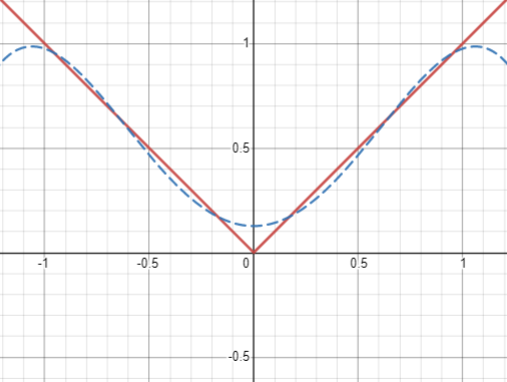
\includegraphics[scale=0.5]{zad1.PNG} \par
\vspace{3mm}
\hfil{Rysunek 1: Wykres funkcji $\left | x \right | oraz \ q(x) $} \par

\vspace{5mm}

\hfil
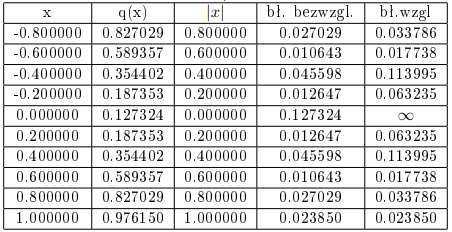
\includegraphics[scale=0.8]{tab11.PNG} \par
\vspace{3mm}


\vspace{5mm}

\subsection{Wykonać aproksymację funkcję  |sin(x)|  funkcjami trygonometrycznymi w zakresie [-pi, pi]}

Funkcja $|\sin x|$ spelnia warunki Dirichleta na podanym przedziale. Ponieważ funkcja jest parzysta, mozna ją rozwinąć w szereg cosinusów:
$$
\begin{array}{l}
\vspace{2mm}
a_{n}=\frac{1}{\pi} \int_{-\pi}^{\pi}|\sin x| \cos n x d x=\frac{-(2(\cos (\pi n)+1))}{\left(\pi\left(n^{2}-1\right)\right)} \\
\vspace{2mm}
a_{n}=\frac{1}{\pi} \int_{-\pi}^{\pi}|\sin x| \cos n x d x=\frac{-\left(2\left((-1)^{n}+1\right)\right)}{\left(\pi\left(n^{2}-1\right)\right)}
\end{array}
$$
dla $n>1$ oraz $a_{1}=0$ dla pozostatych nieparzystych $n, a_{n}=0$ bo $(-1)^{n}+1=0$. Dla parzystych $n$ licznik jest równy -4 , więc dla parzystych $n$ prawdziwy jest wzór $a_{n}=\frac{-4}{\pi\left(n^{2}-1\right)}$


$$
\begin{array}{c}
\vspace{2mm}
\frac{a_{0}}{2}=\frac{2}{\pi} \\
\vspace{2mm}
S_{N}(x)=\frac{2}{\pi}+\sum_{n=1}^{N} a_{n} \cos n x \\
\vspace{2mm}
a_{2}=\frac{-4}{3 \pi} \\
\vspace{2mm}
a_{4}=\frac{-4}{15 \pi} \\
\vspace{2mm}
a_{6}=\frac{-4}{35 \pi} \\
\vspace{2mm}
S_{6}(x)=\frac{2}{\pi}-\frac{4}{3 \pi} \cdot \cos (2 x)-\frac{4}{15 \pi} \cdot \cos (4 x)-\frac{4}{35 \pi} \cdot \cos (6 x)
\end{array}
$$


\hfil
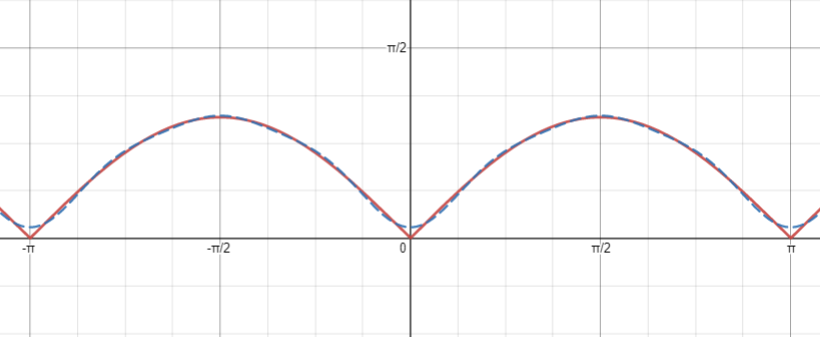
\includegraphics[scale=0.5]{lab3sin.png} \par
\vspace{3mm}
\hfil{Rysunek 2: Wykresy funkcji $\left | sin(x) \right | oraz \ S_{6} $} \par

\vspace{5mm}


\section{Bibliografia}

\begin{enumerate}
  \item \url{http://home.agh.edu.pl/~funika/mownit/lab3/aproksymacja.pdf}
  \item \url{https://pl.wikipedia.org/wiki/Szereg_Fouriera}
\end{enumerate}

\end{document}
